\documentclass{standalone}
\usepackage{tikz}
\begin{document}
    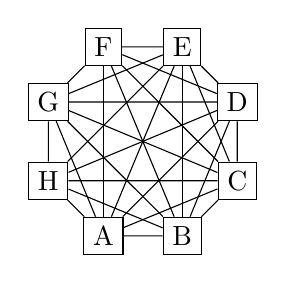
\begin{tikzpicture}
      \node[draw] (a) at (0,.3) {A};
      \node[draw] (b) at (1,.3) {B};
      \node[draw] (c) at (1.7,1) {C};
      \node[draw] (d) at (1.7,2) {D};
      \node[draw] (e) at (1,2.7) {E};
      \node[draw] (f) at (0,2.7) {F};
      \node[draw] (g) at (-.7,2) {G};
      \node[draw] (h) at (-.7,1) {H};
      \draw (a) -- (b) -- (c) -- (d) -- (e) -- (f) -- (g) -- (h) -- (a);
      \draw (a) -- (c) -- (h) -- (d) -- (g) -- (e);
      \draw (b) -- (h);
      \draw (b) -- (f);
      \draw (b) -- (d);
      \draw (b) -- (g);
      \draw (b) -- (e);
      \draw (h) -- (e);
      \draw (d) -- (f);
      \draw (g) -- (c);
      \draw (a) -- (d);
      \draw (a) -- (e);
      \draw (a) -- (f);
      \draw (a) -- (g);
      \draw (e) -- (c);
      \draw (c) -- (f);
    \end{tikzpicture}
\end{document}
%%% Local Variables: 
%%% mode: latex
%%% TeX-master: t
%%% End: 
